\begin{figure*}[tbh!]
\centering
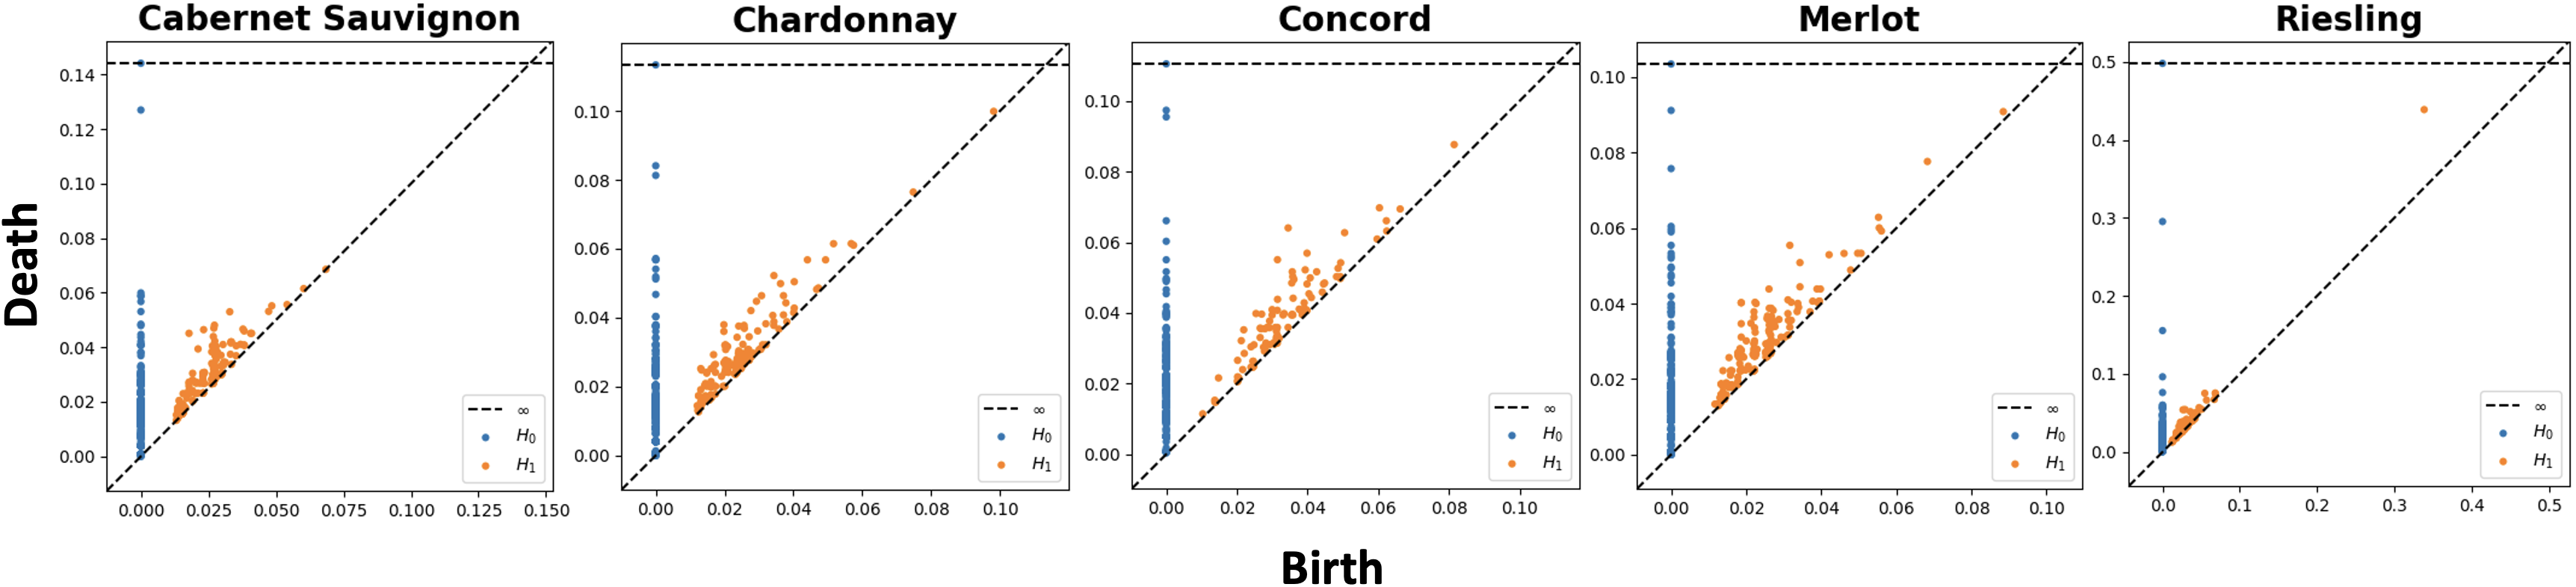
\includegraphics[width=2.1\columnwidth]{Figures/CultivarsPD.png} 
\caption{Persistence diagrams for the five grape cultivars, each constructed using their data from seasons 1999 through 2022.
Blue and orange dots represent connected components ($\mathrm{dgm}_0$) and holes ($\mathrm{dgm}_1$) respectively. The vertical distance of a dot from the main diagonal corresponds to the feature's duration. 
}
\label{fig:cultivarspd}
\end{figure*}

\begin{figure*}[tbh]
\centering
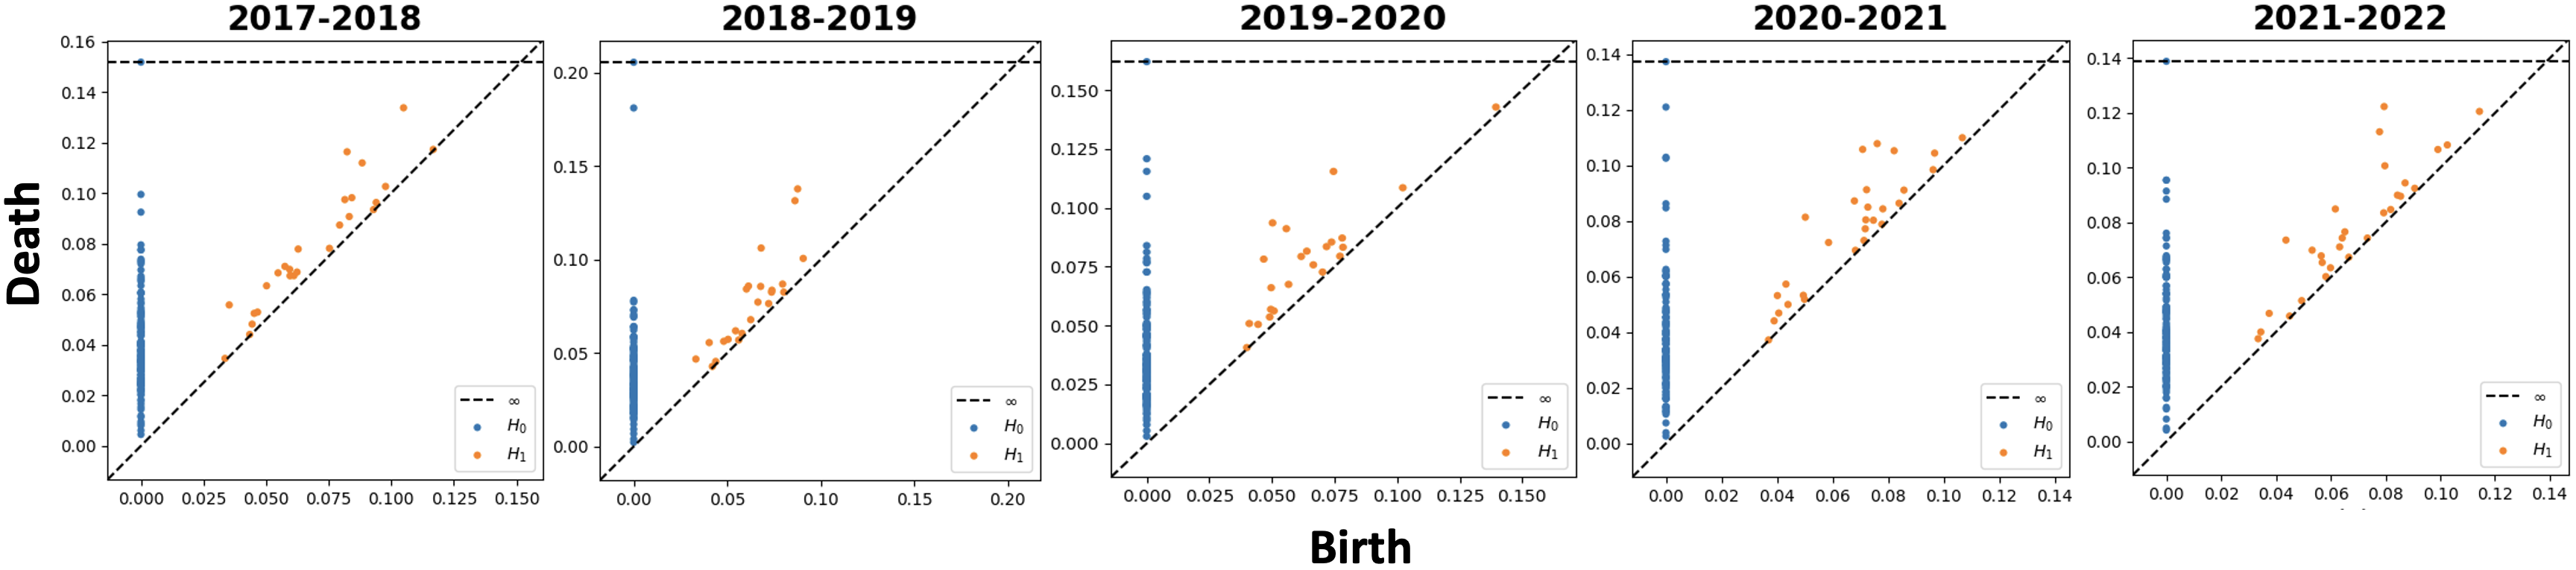
\includegraphics[width=2.1\columnwidth]{Figures/SeasonsPD.png} 
\caption{Persistence diagrams for the last 5 seasons of the cold hardiness data. Each diagram is for one season, constructed using all 5 cultivar data for that season.
}
\label{fig:PDpairseasons}
\end{figure*}


\section{Results}
\label{sec:results}

In this section, we present the results of applying our methodology described under Tasks 1 and 2 in Section~\ref{sec:PDforCH} on the grape cold hardiness data set described in Section~\ref{sec:data}.
All experiments shown are for  $LTE_{50}$ values (due to space restrictions). 
All persistence diagrams and Wasserstein distances were computed using the \texttt{Scikit-TDA} package \cite{scikittda2019}. 
%\todo{add citation}

\paragraph{Results of Inter-cultivar Comparisons:}
\label{sec:results:intercultivar}
%First we show the results of inter-cultivar analysis. The results were obtained using the methodology described in Task 1 of Section~\ref{sec:PDforCH}.
Figure~\ref{fig:cultivarspd} shows the persistence diagrams computed for each cultivar, and
Table~\ref{tab:distance_matrix_cultivars} shows the Wasserstein distance matrix for all cultivar pairs using their persistence diagrams.
As can be seen, CD and MR display the largest distance, while CH and CS constitute the closest pair.
WR (Riesling) has a larger distance to all other cultivars except to CD. 
Note that there are no known connections between the cold hardiness trait and the consumptive type of grape (i.e., wine or juice or table).


\begin{table}[htb]
\centering
\resizebox{0.7\columnwidth}{!}{
\begin{tabular}{ |l|r|r|r|r|r|}
\hline
&	\multicolumn{1}{|c|}{\textbf{CD}}	&	\multicolumn{1}{|c|}{\textbf{CH}}	&	\multicolumn{1}{|c|}{\textbf{CS}}	&	\multicolumn{1}{|c|}{\textbf{MR}}	&	\multicolumn{1}{|c|}{\textbf{WR}}\\\hline
\textbf{CD}	&	0	&	0.236	&	0.201	&	\emph{0.305}	&	0.168\\\hline
\textbf{CH}	&	0.236	&	0	&	\emph{0.146}	&	0.164	&	0.233\\\hline
\textbf{CS}	&	0.201	&	0.146	&	0	&	0.168	&	0.206\\\hline
\textbf{MR}	&	0.305	&	0.164	&	0.168	&	0	&	0.286\\\hline
\textbf{WR}	&	0.168	&	0.233	&	0.206	&	0.286 &	0\\\hline
\end{tabular}
}
\caption{Pairwise distance matrix for cultivars. For each cultivar data from 1999-2022 was used. Each value shows the Wasserstein distance between the $\mathrm{dgm}_1$ obtained for the corresponding two cultivars.
}
\label{tab:distance_matrix_cultivars}
\end{table}

\vspace*{-0.2in}
\paragraph{Results of Intra-cultivar Variability:}
\label{sec:results:intracultivar}
Next, we ask how variable is each cultivar across the different seasons. This is captured by the level of branching observed within the $\mathrm{dgm}_1$ for that cultivar (Task 1, Section~\ref{sec:PDforCH}).
Figure~\ref{fig:cultivarspd}
shows all five persistence diagrams. As can be readily observed, each cultivar has a different profile. 
Intuitively, if a cultivar behaves highly variable from season to season, we can expect to see more branching. However, if those branching events are relatively short-lived, then they correspond to small time scale variations. Longer lived branching events correspond to more persistent divergent behavior. 
From Figure~\ref{fig:cultivarspd}, it can be seen that all three of CH, CD, and MR show numerous holes of wide ranging durations. In contrast, CS and WR show fewer holes with smaller duration. This suggests that CS and WR are less variable compared to the other varieties.



\paragraph{Seasonal comparisons:}
\label{sec:results:seasonalcompare}
We also compared the different seasons (from 1999 to 2022) using the methodology described in Task 2 of Section~\ref{sec:PDforCH}.
Figure~\ref{fig:PDpairseasons} shows the persistence diagrams for only the last 5 seasons (due to space constraints).
We observed that the two most different seasons (i.e., with the largest Wasserstein distance) were the seasons 2001-2002 vs. 2010-2011 (shown 
in Figure~\ref{fig:holesseason}). 


%The following observations can be made. a) The distance values range within a tight interval of [0.070, 0.101], with an average of 0.088. b) The largest distance was observed between the season pairs 2017-2018 vs. 2019-2020, while the smallest was for 2017-2018 vs. 2021-2022. c) On an average though, the season 2018-2019 showed the maximum distance from all other seasons.  This can be easily confirmed by visually inspecting the persistence diagrams shown for all 5 seasons in Figure~\ref{fig:PDpairseasons}.







%\begin{figure*}[tbh]
%\centering
%\begin{subfigure}{.53\textwidth}
%  \centering
%  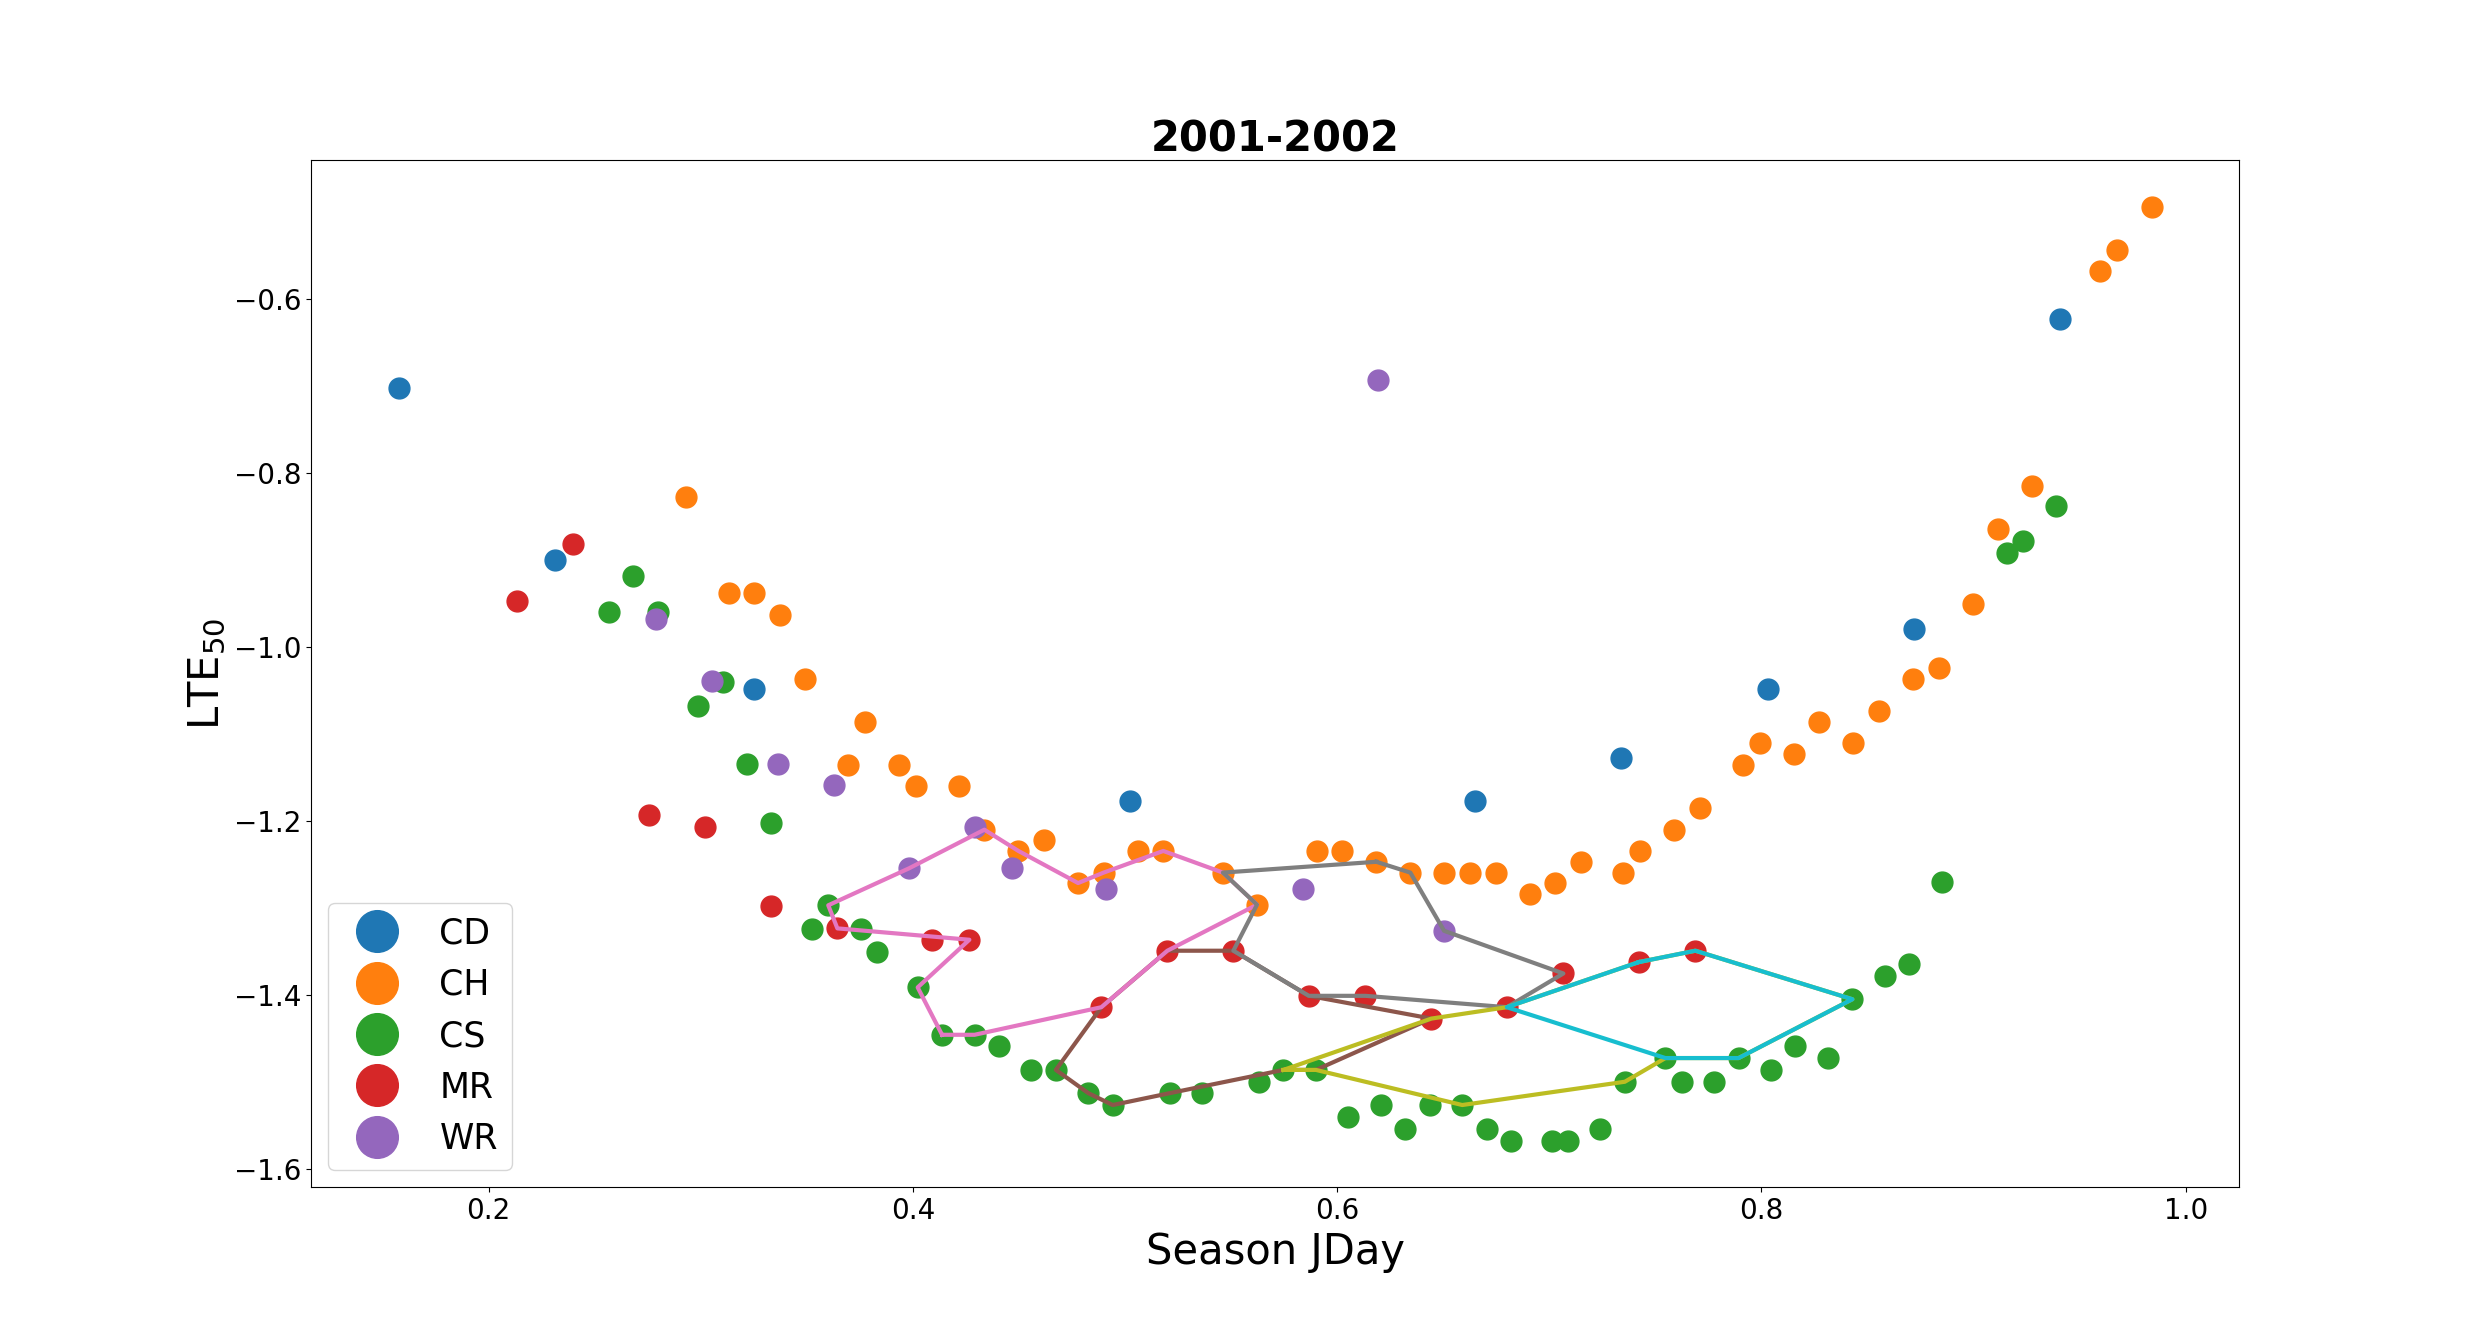
\includegraphics[width=1\linewidth]{Figures/2001-2002All.png}
%  \caption{A subfigure}
%  \label{fig:sub1}
%\end{subfigure}%
%\begin{subfigure}{.53\textwidth}
%  \centering
%  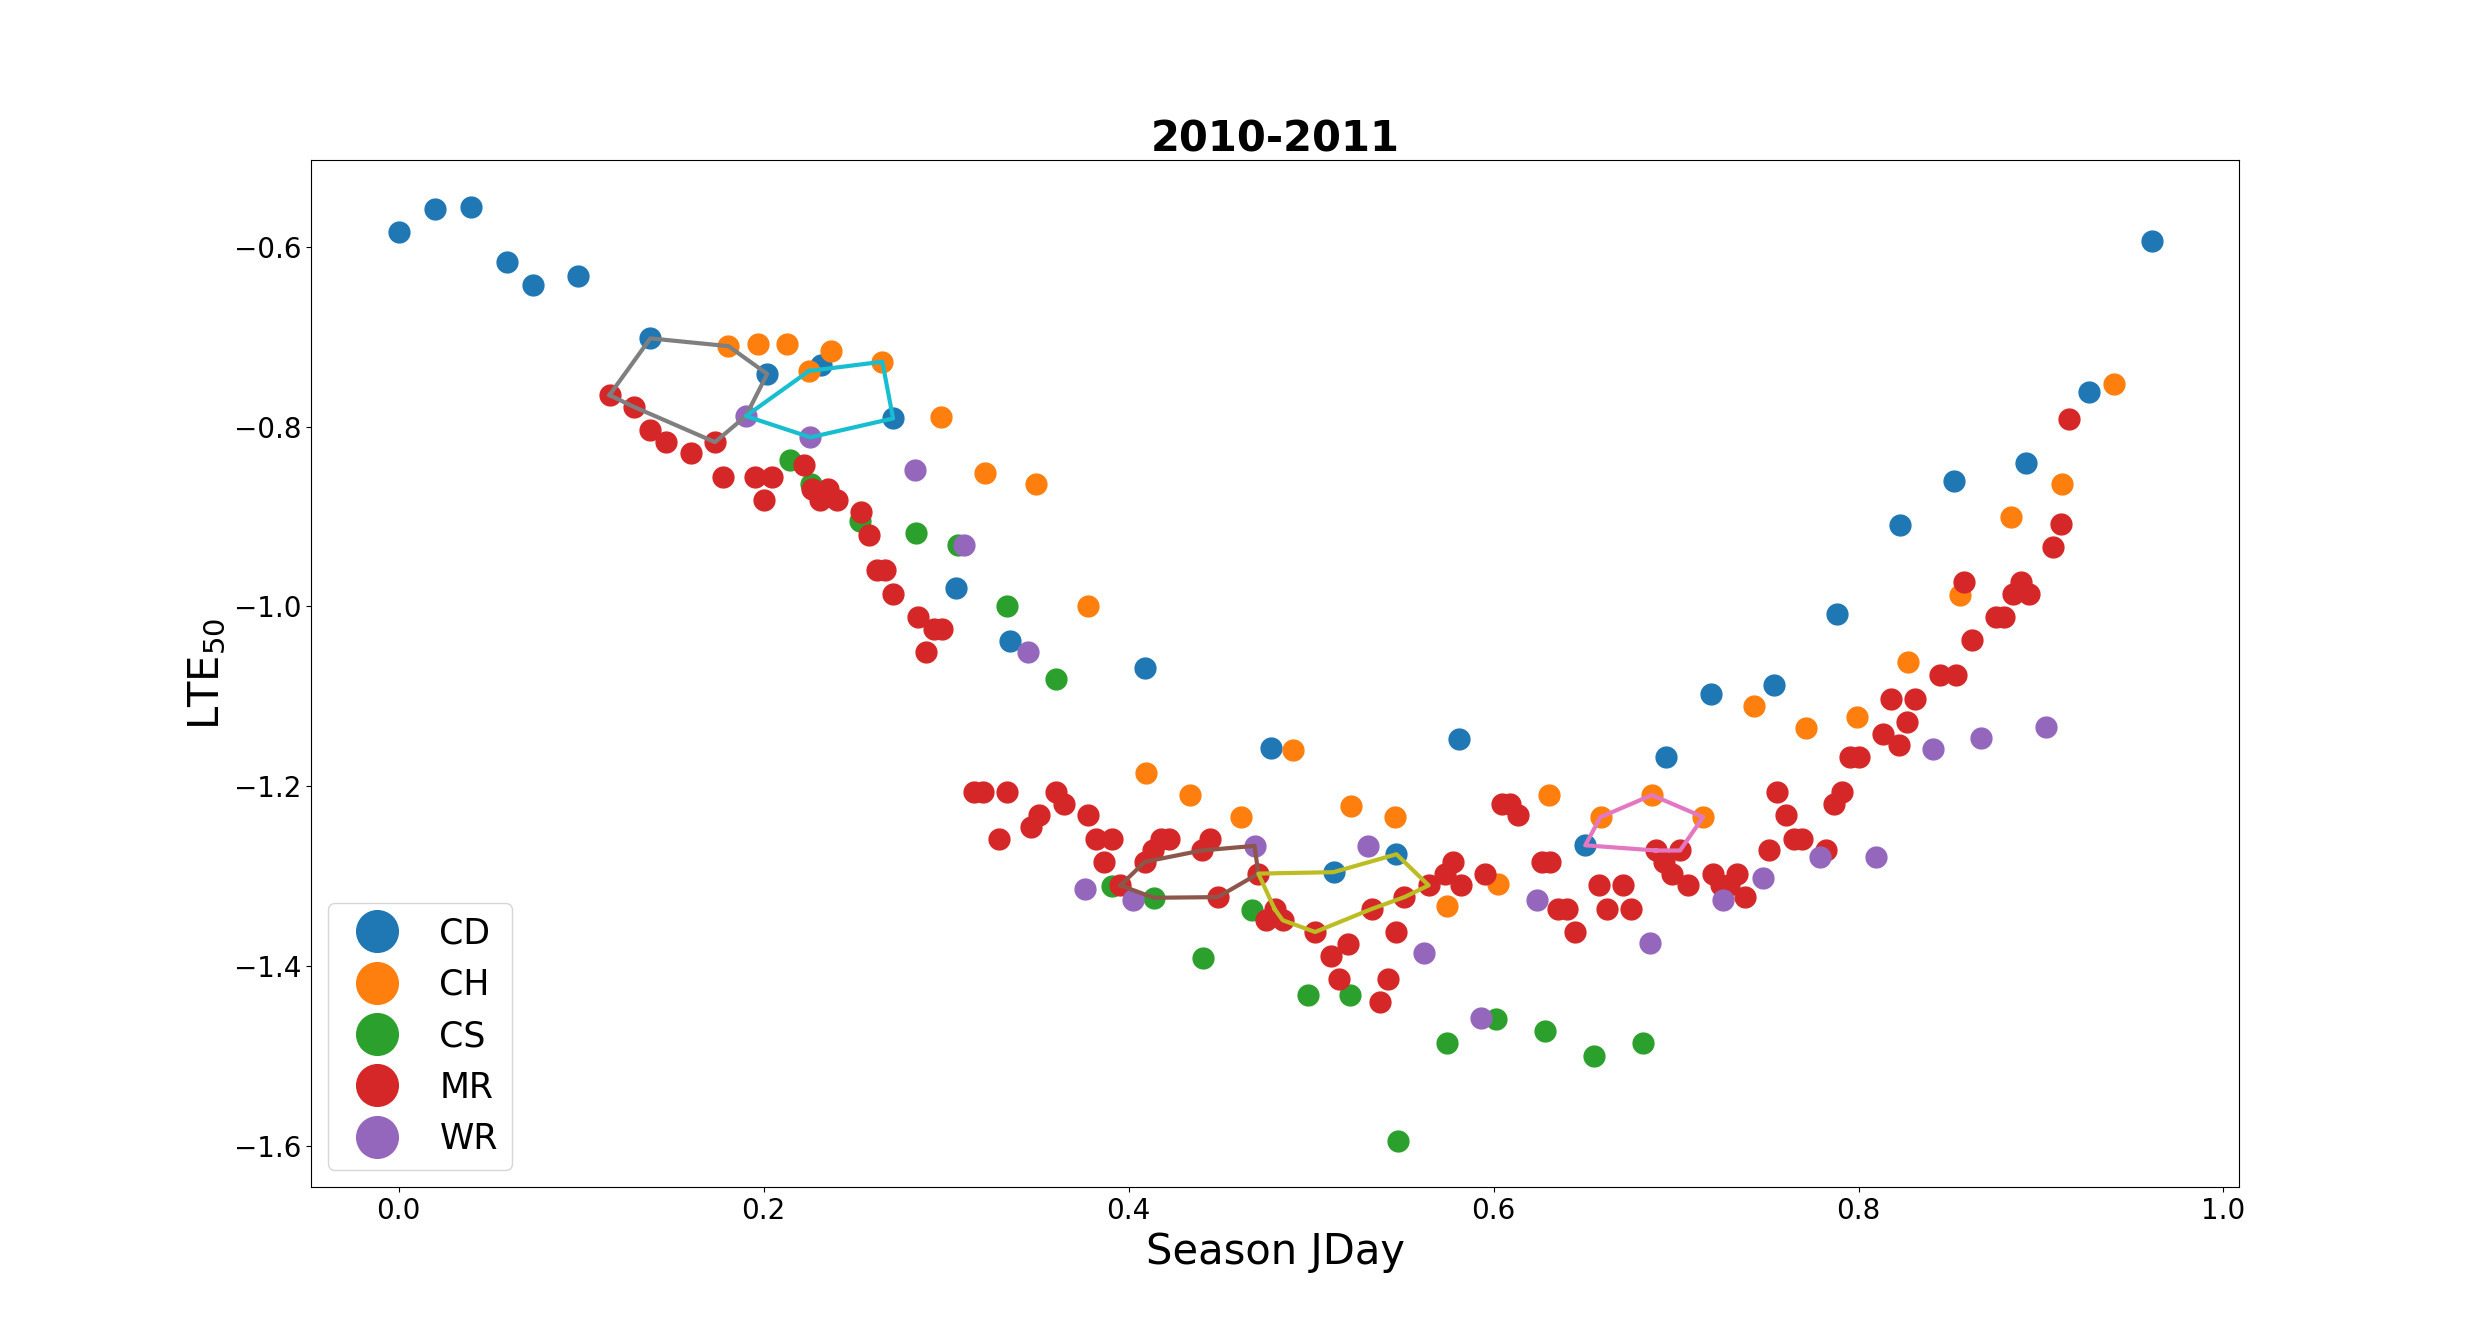
\includegraphics[width=1\linewidth]{Figures/2010-2011All.png}
%  \caption{A subfigure}
%  \label{fig:sub2}
%\end{subfigure}
%\caption{A figure with two subfigures}
%\label{fig:test}
%\end{figure*}


%Point cloud of data for all five cultivars analyzed for each available year/season. We used persistent homology, as implemented in the \texttt{cyclonysus} tool \cite{cyclonysus}, to generate the cycles or loops present in the point cloud. Loops in such a point cloud symbolize a branching event. It means that certain cultivars diverged from the others for a time period before merging with the others. We filtered the branching events to only include ones with multiple cultivars. 
%We also analyzed these branching events to investigate whether there is consistency in the branching events. Information about which cultivars were part of the cycles was also collected. We also collected data about the relative timing of the branching events with respect to the season. Across cultivars, we saw that the differences between cultivars start to appear at about JDAY 347 and end at about JDAY 490.

%\subsubsection{Pick the two most different seasons and explain how they are different}
%To inspect how intercultivar branching differed across seasons we compared all the available seasons with each other. We first generated persistence diagrams of each season for point clouds with all five cultivars and then computed the Wasserstein distance for each possible pair. We picked the pair with the greatest Wasserstein distance (0.17887) We can see that the two seasons have extremely different branching events with respect to the span and cultivars involved.  

%\subsubsection{Querying by time window within each season}
%- select March 
%- out of 20 years, 10 years (C1 and C2 were part of the same loop - hence different), 5 years (C2 and C3 were different)

\begin{comment}

\begin{table}[bhp]
\centering
\resizebox{1\columnwidth}{!}{
\begin{tabular}{ |c|r|r|r|r|}
\hline
\multicolumn{1}{|c|}{\textbf{Cultivar}} &\makecell{\textbf{Number of} \\ \textbf{branching events*}} &\multicolumn{1}{|c|}{\textbf{Avg. Span}} &\multicolumn{1}{|c|}{\textbf{Avg. Start JDAY}} &\multicolumn{1}{|c|}{\textbf{Avg. End JDAY}}\\\hline
CS &77 &45.026 &344.844 &389.870\\\hline
CH &83 &41.398 &347.193 &388.590\\\hline
CD &49 &41.061 &343.939 &385.0\\\hline
MR &106 &43.283 &349.953 &393.236\\\hline
WR &80 &43.763 &344.45 &388.213\\\hline
\end{tabular}
}
\caption{Summary of results. *The number represents the times a cultivar was part of a hole.}
\label{tab:results}
\end{table}
\end{comment}





